\documentclass[8pt]{extarticle}
\usepackage{multicol,caption}
\usepackage[utf8]{inputenc}
\usepackage[english]{babel}
\usepackage[a4paper, landscape, margin=1cm, footskip=0.7cm]{geometry}
\usepackage{graphicx}
\usepackage{lipsum}
\usepackage{amsmath}
\usepackage{dsfont}
\usepackage{gensymb}
\usepackage{mathrsfs}
\usepackage{framed}
\usepackage{enumerate}
\usepackage{array}
\usepackage{datetime}
\usepackage{calligra}
\usepackage[dvipsnames]{xcolor}
\usepackage[titles]{tocloft}
\usepackage[sfdefault]{roboto}
\usepackage{enumitem}
\usepackage[compact]{titlesec}


\setenumerate{itemsep=0pt,topsep=0pt}
\setitemize{itemsep=0pt, topsep=0pt}

\setlength{\parskip}{0cm}
\setlength{\parindent}{0em}
%\setlength{\headsep}{0pt}
\setlength{\topskip}{0pt}
%\setlength{\topmargin}{0pt}
\setlength{\topsep}{0pt}
\setlength{\partopsep}{0pt}

%% TOC
\graphicspath{{figures/}}

\makeatletter
\newenvironment{Table}
   {\par\bigskip\noindent\minipage{\columnwidth}\centering}
   {\endminipage\par\bigskip}
\makeatother

\setlist{nolistsep}


\newenvironment{Figure}
  {\par\medskip\noindent\minipage{\linewidth}}
  {\endminipage\par\medskip}

\newenvironment{conditions}
{\par\vspace{\abovedisplayskip}\noindent\begin{tabular}{>{$}l<{$} @{${}={}$} l}}
{\end{tabular}\par\vspace{\belowdisplayskip}}

\setlength{\columnseprule}{0.2pt}
\setlength{\columnsep}{10pt}
\renewcommand{\columnseprulecolor}{\color{lightgray}}

% TOC
\setlength{\cftbeforesecskip}{-.2ex}



\begin{document}

\begin{multicols}{3}
\noindent
\large IT Systems Management
\normalsize \\
\today, \currenttime
\vspace{-1.2em}\\
{\small\tableofcontents}

\section{Executive Support} 
Crucial for SysMan. Business metrics is a good argument for Ex. Supp., continuous support
should be ensured. \\

\section{Organizing for Systems Management}
\subsection{Factors to Consider in Designing IT Organizations}
In the case of IT, restructuring is often necessary to support company growth, increased customer demand, 
changing business requirements, acquisitions, mergers, buyouts, or other industry changes.
Three key factors by which infrastructures can be organized: 
departmental responsibilities, planning orientation, and systems management processes.
\paragraph{Org. Model} Know Your Business (KYB), Locating Deparments in the Infrastructure, Identify Process Owners.

\section{Staffing for System Management}
Skilled professionals are needed at the outset to develop plans, design processes, and evaluate technologies; 
then they are needed to transform these ideas from paper into realities.

\paragraph{Skill Set} defined as technical familiarity with a particular software product, architecture, or platform.
\paragraph{Skill Level} defined as the length of experience and depth of technical expertise and variety of platform
familiarity an individual has acquired and can apply to a given technology.

\paragraph{Importance of the right staff} Determining required skill sets and skills levels, assessing skill levels of
current onboard staff (alternative sources of staffing, recruiting infra. staff from 
the outside [operative/consultive]), selecting the \textit{Most Qualified Candidate},
retaining \textit{Key Personnel}, using \textit{Consultants and Contractors} 
(benefits / drawbacks are involved, steps for developing career paths for staff memebers)

\section{Ethics, Legislation, and Outsourcing}
\paragraph{Personal Ethics} Set values an individual uses to influence and guide his or her personal behavior.
\paragraph{Business Ethics} Set values an individual uses to influence and guide his or her business behavior.
Business ethics tend to focus on the behaviors of an individual as it pertains to his or her work environment.
The differences between personal and business ethics may be at once both subtle and far-reaching.

\paragraph{NPI} Stands for non-public information and pertains to the private, 
personal information of an individual not readily available in public records. 
Customers typically disclose such information to private or public companies to transact business. 
Examples of NPI are social security numbers, unlisted telephone numbers, and credit card account numbers.

\section{Customer Service}
IT evolved into a service organization. 
\begin{itemize}
\item Identifying your key customers
\item Identifying key services of key customers
\item Identifying key processes that support key services
\item Identifying key suppliers that support key processes
\end{itemize}
Integrating the 4 key elements of Good Customer Service.
\section{Availability}
\paragraph{Availability} Process of optimizing the readiness of production systems by accurately
 measuring, analyzing, and reducing outages to those production systems. \\
The ratio of the {\color{MidnightBlue}{total time a functional unit is capable of being
used during a given interval}} to {\color{MidnightBlue}{the length of the interval}}. \\
Mean Time To Failure (MTTF), Mean Time To Repair (MTTR)
\paragraph{Responsiveness} Operational responsiveness is a quality of a business process or supporting IT solution, 
which indicates its ability to respond to changing conditions and customer interactions as they occur.  
\paragraph{Uptime} measure of the time that individual components within a production system are functionally operating.
This contrasts to availability, which focuses on the production system as a whole.

\paragraph{Slow Response} refers to unacceptably long periods of time for an online transaction to complete processing 
and return results to the user. 
The period of time deemed unacceptable varies depending on the type of transaction involved. 
For simple inquiries, a one-second response may seem slow; for complex computations, 
two- or three-second responses may be acceptable. Slow response is usually a performance and tuning problem requiring 
highly-trained personnel with specialized expertise

\paragraph{Downtime} Downtime refers to the total inoperability of a hardware device, a software routine, or some other
critical component of a system that results in the outage of a production application.

\paragraph{High Availability} refers to the design of a production environment such that all single points of failure 
are removed through redundancy to eliminate production outages. 
This type of environment is often referred to as being fault tolerant.

\paragraph{SMART} \textbf{S}pecific, \textit{Targets should be straightforward and emphasize what you want to happen}.
\textbf{M}easurable, \textit{If a target cannot be measured then you cannot determine whether it has been
achieved}. \textbf{A}chievable, \textit{It must be possible to achieve the target with an acceptable investment of time
and resources}. \textbf{R}elevant, \textit{Achieving the target must contribute to the overall business mission}.
\textbf{T}imely, \textit{The target must be something that can be achieved and measured over the
reporting period of the SLA\footnote{SLA is short for service level agreement and refers to a documented, 
negotiated agreement between a representative from an IT department and a representative from an end-user department 
concerning the quality of service delivered. 
Common SLA metrics include percent uptime availability, average response times, 
and escalation procedures for problems.}}.

\subsection{7-R{\small s} of availability}
These seven Rs of high availability all contribute in a unique way to extending uptime, minimizing downtime,
and improving the overall level of service provided by online systems.

\subsubsection{Redundancy}
Power Supply, Multiple processors, Segmented Memory, Redundant Disks
\subsubsection{Reputation}
The reputation of key suppliers of servers, disk storage systems, database management systems, and network hardware and
software plays a principle role in striving for high availability.
It is always best to go with the best. Reputations can be verified in several ways, including the following: Percent 
of market share, Reports from industry analysts such as Gartner Group, Publications such Wall Street Journal and
ComputerWorld, Track record of reliability and repairability, Customer references

\subsubsection{Reliability}
The reliability of the hardware and software can also be verified from customer 
references and industry analysts. 
Beyond that, you should consider performing what we call an empirical component reliability analysis.
The following list describes the seven steps required to accomplish this.

\begin{enumerate}
    \item Review and analyze problem management logs.
    \item Review and analyze supplier logs.
    \item Acquire feedback from operations personnel.
    \item Acquire feedback from support personnel.
    \item Acquire feedback from supplier repair personnel.
    \item Compare experiences with other shops.
    \item Study reports from industry analysts.
\end{enumerate}


\subsubsection{Repairability}
This refers to is the relative ease with which service technicians can resolve or replace failing components. 
A common metric used to evaluate this trait is the average or mean time to repair (MTTR).
MTTR is sometimes interpreted as the mean time to recover, the mean time to restore, or the mean time to resolve. 
It measures the average time it takes to do the actual repair.
$\text{MTTR} = \frac{\text{sum of repair times}}{\text{\# of failures}}$
\subsubsection{Recoverability}
This refers to the ability to overcome a momentary failure in such a way that there is no impact on end-user 
availability. 
It could be as small as a portion of main memory recovering from a single-bit memory error; 
it can be as large as having an entire server system switch over to its standby system with no loss of data or 
transactions. 
Recoverability also includes retries of attempted reads and writes out to disk or tape, as well as the retrying of 
transmissions down network lines.
\subsubsection{Responsiveness}
This trait is the sense of urgency all people involved with high availability need to exhibit. 
This includes having well-trained suppliers and in-house support personnel who can respond to problems quickly and 
efficiently. 
It also pertains to how quickly the automated recovery of resources such as disks or servers can be enacted.
Escalation is another aspect of responsiveness that ensures higher levels of technical expertise and management support
are involved to restore availability as quickly as possible. 
Escalation guidelines are usually documented in service-level agreements between IT and business customers.

\subsubsection{Robustness}
A robust process will be able to withstand a variety of forces—both internal and external—that could easily disrupt 
and undermine availability in a weaker environment. 
Robustness puts a high premium on documentation and training to withstand the following:
\paragraph{Technical Changes as they relate to} Platforms, Products, Services, Customers
\paragraph{Personnel Changes as they relate to} Turnover, Expansion, Rotation
\paragraph{Business changes as they relate to} New direction, Acquisitions, Mergers

Defining a process to measure and monitor Infrastructure's Availability: Committed Hours of Availability (A),
Outage hours (B), Achieved Availability: $\frac{A-B}{A} \cdot 100 \%$.

\section{Performance and Tuning}
Methodology to maximize throughput and minimize response times of batch jobs,
online transactions, and Internet activities.
The five infrastructure areas most impacted by performance and tuning are:
\begin{itemize}
    \item Servers
    \item Disk storage
    \item Databases
    \item Networks
    \item Desktop Computers
\end{itemize}
\section{Production Acceptance}
Methodology used to consistently and successfully deploy application systems into a 
production environment regardless of platform.

\paragraph{Consistent methodology} While the methodology is consistent, it is not necessarily identical across all 
platforms. This means there are essential steps of the process that need to be done for every production deployment, 
and then there are other steps that can be added, omitted, or modified depending on the type of platform selected 
for production use.
 
\paragraph{Deploying into a production environment} This implies that the process is not complete until all users are 
fully up and running on the new system. For large applications, this could involve thousands of users phased in over
several months.
 
\paragraph{Application system} This refers to any group of software programs necessary for conducting a company’s
business—the end-users of which are primarily, but not necessarily, in departments outside of IT. 
This excludes software still in development, as well as software used as tools for IT support groups.

\paragraph{Production Acceptance Process}
\begin{enumerate}
\item Identify an Executive Sponsor
\item Select a Process Owner
\item Solicit Executive Support
\item Assemble a Production Acceptance Team
\item Identify and Prioritize Requirements
\item Develop Policy Statements
\item Nominate a Pilot System
\item Design Appropriate Forms
\item Document updates, extension and new procedures
\item Run field tests and a solid pilot phase
\item Revise Policies, Procedures, and Forms
\item Define an adequate marketing strategy (if applicable)
\item Conduct a lessons-learned sessions
\item Follow-up with continuous improvements
\end{enumerate}
\noindent
Pay attention:
\begin{itemize}
\item Production Acceptance is not Change Management
\item New Applications vs. New Versions of Existing Applications
\end{itemize}

\section{Change Management}
Change Management is the process to control and coordinate all changes to an IT production environment. 
Control involves requesting, prioritizing, and approving changes; coordination involves collaborating, scheduling,
communicating, and implementing changes. \\
A change is defined as any modification that could impact the stability or responsiveness of an
IT production environment.

\begin{center}
    \begin{minipage}{\columnwidth}
        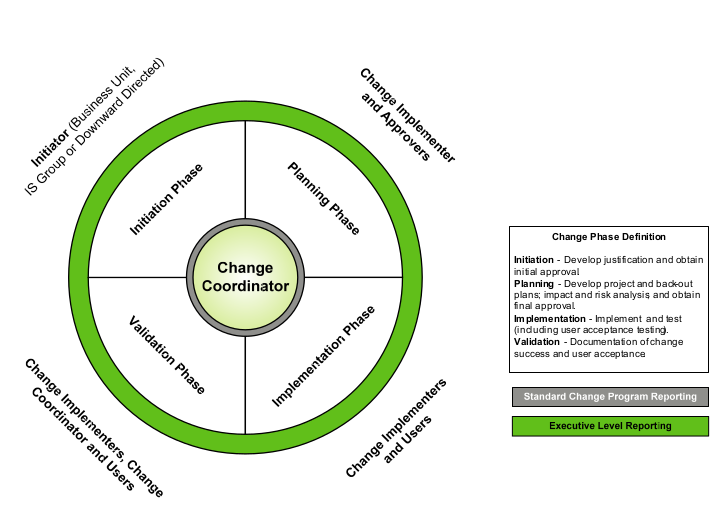
\includegraphics[width=\columnwidth]{change-coordinator.png}
    \end{minipage}
\end{center}

\subsection{Key Steps Required in Developing a Change Management Process}
\begin{enumerate}
\item Identify an executive sponsor.
\item Assign a process owner.
\item Select a cross-functional process design team.
\item Arrange for meetings of the cross-functional process design team.
\item Establish roles and responsibilities for members supporting the design team.
\item Identify the benefits of a change management process.
\item If change metrics exist, collect and analyze them; if not, set up a process to do so.
\item Identify and prioritize requirements.
\item Develop definitions of key terms.
\item Design the initial change management process.
\item Develop policy statements.
\item Develop a charter for a Change Advisory Board (CAB).
\item Use the CAB to continually refine and improve the change management process.
\end{enumerate}

\subsection{Scope}
Because the Change Management Process deals with the management of changes in the production
environment, it is imperative that both customers and the company’s change organization understand the
events that are considered within the scope of the process. In this section, the scope is described and
includes areas which are both within and outside of the change management process scope.

\subsubsection{Tasks in the scope of CMP}
\begin{itemize}
\item SDLC – Changes handled through the formal software development life cycle will be included within the 
company’s change management program.
\item Hardware – Installation, modification, removal or relocation of computing equipment.
\item Software – Installation, patching, upgrade or removal of software products including operating systems, access methods, commercial off-the-shelf (COTS) packages, internally developed packages and utilities.
\item Database – Changes to databases or files such as additions, reorganizations and major maintenance.
\item Application – Application changes being promoted to production as well as the integration of new application systems and the removal of obsolete elements.
\item Moves, Adds, Changes and Deletes – Changes to system configuration.
\item Scheduled Changes - Requests for creation, deletion, or revision to job schedules, back-up schedules or other regularly scheduled jobs managed by the IT department.
\item Telephony – Installation, modification, de-installation, or relocation of PBX/VOIP equipment and services.
\item Desktop – Any modification or relocation of desktop equipment and services for users or classroom labs.
\item Generic and Miscellaneous Changes – Any changes that are required to complete tasks associated with normal job requirements.
\end{itemize}

\subsubsection{Tasks that aren't part of CMP}
\begin{itemize}
    \item Contingency/Disaster Recovery
    \item BCM related activities
    \item Changes to non-production elements or resources
    \item Changes made within the daily administrative process.
        \begin{itemize}
        \item Password resets
        \item User adds/deletes
        \item User modifications
        \item Adding, deleting or revising security groups
        \item Rebooting machines when there is no change to the
        \item configuration of the system
        \item File permission changes
        \end{itemize}
\end{itemize}

\subsection{Workflow Tasks}
\begin{center}
    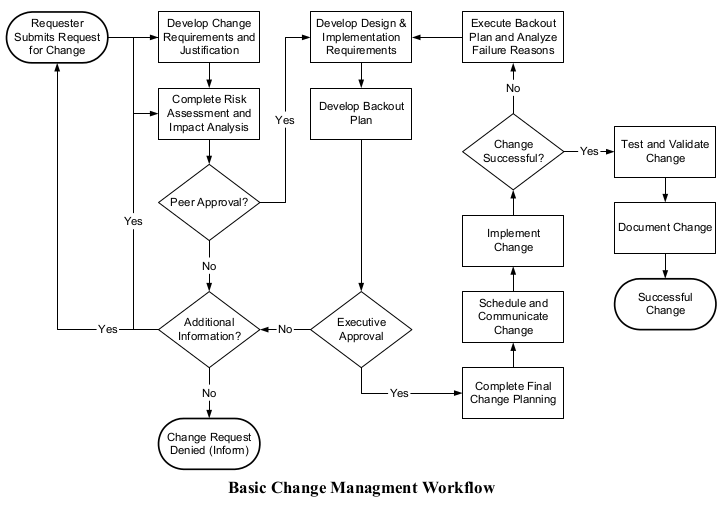
\includegraphics[width=\columnwidth]{basic-change-management-workflow.png}
\end{center}

\subsection{Approvals Required for Change Based on Risk Level}
\begin{center}
    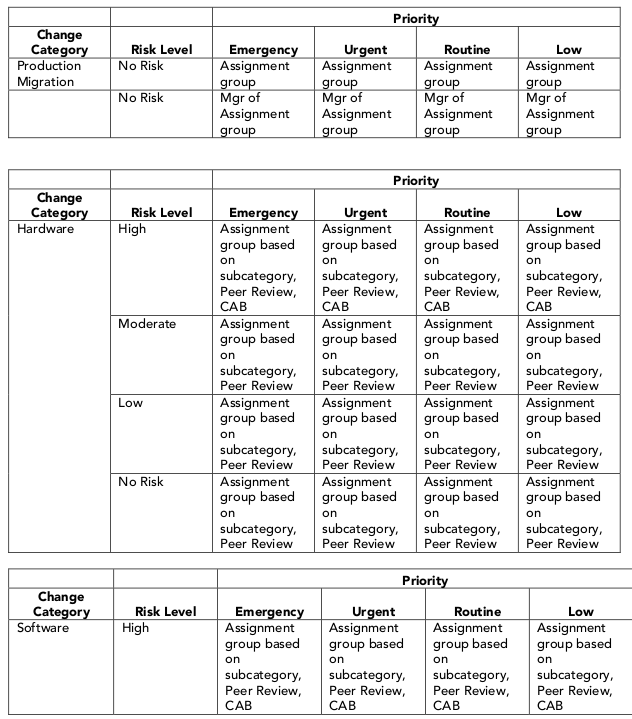
\includegraphics[width=\columnwidth]{approval-required-change-based-on-risk-level.png}
\end{center}

\subsection{Risk Level Based Lead Times}
It is essential that requests for change are submitted and approved in a timely manner. This will allow
completion of accurate documentation, change processing and obtaining the approvals in sufficient time
prior to the requested implementation date.
Lead times are the number of days an action (Initiation or Approval) must be completed prior to the
requested implementation date. The number of days will vary, depending on the priority and the risk
level.
\begin{center}
    \begin{minipage}{\columnwidth}
        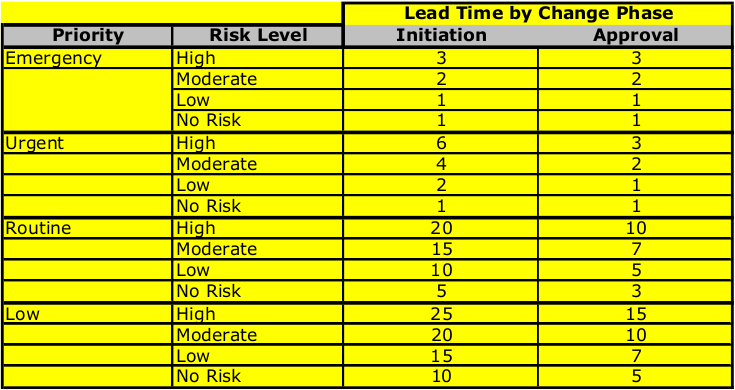
\includegraphics[width=\columnwidth]{risk-based-lead-times.png}
    \end{minipage}
\end{center}

\subsection{Change Approval Phase}
After a minor, major or significant change has been correctly prioritized, categorized, and analyzed by the
Change Coordinator and been through the Peer Review process, the change must be authorized for
implementation. The diagram below identifies the workflow associated with change management
approval at the company:
\begin{center}
    \begin{minipage}{\columnwidth}
        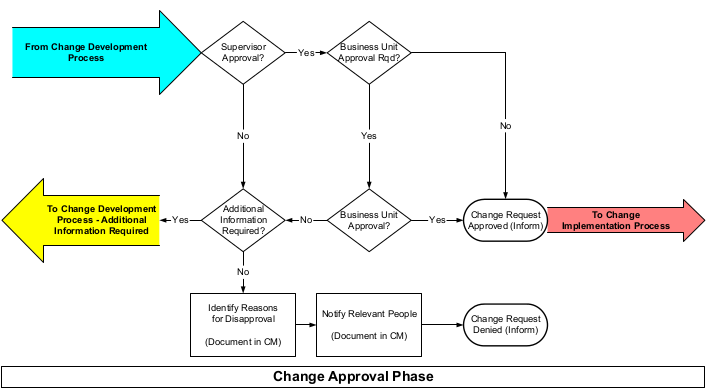
\includegraphics[width=\columnwidth]{change-approval-phase.png}
    \end{minipage}
\end{center}

\subsection{Implementation and Documentation phase}
\begin{center}
    \begin{minipage}{\columnwidth}
        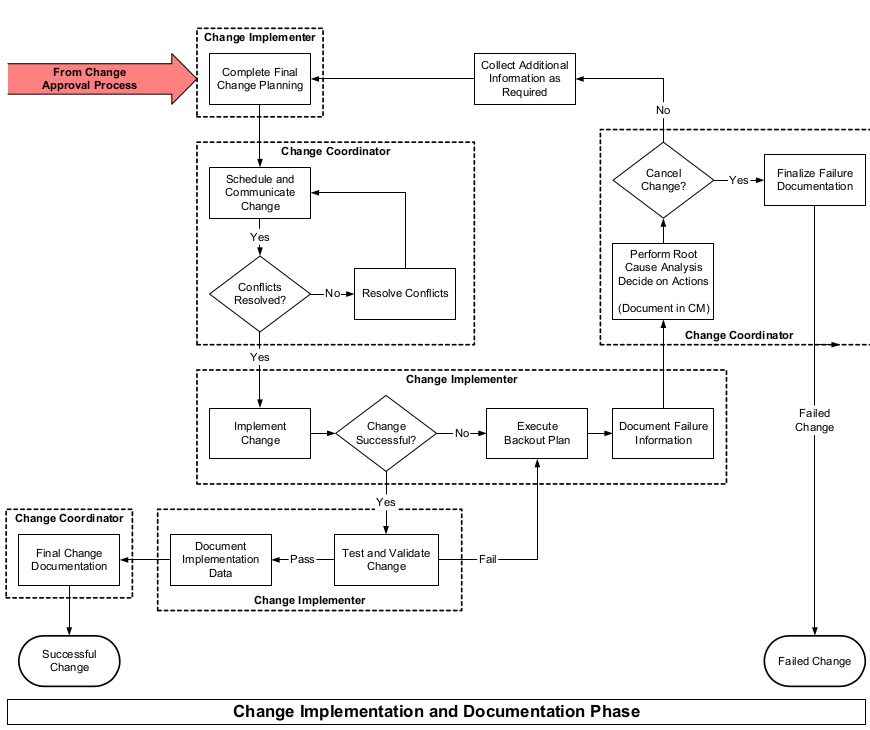
\includegraphics[width=\columnwidth]{change-implementation-documentation-phase.png}
    \end{minipage}
\end{center}

\subsection{Key Definitions}
    \paragraph{Change Advisory Board (CAB)} The CAB is a cross-functional group set up to evaluate change requests
    for business need, priority, cost/benefit, and potential impacts to other systems or processes. Typically
    the CAB will make recommendations for implementation, further analysis, deferment, or cancellation.
    \paragraph{CAB Emergency Committee (CAB/EC)} This is a subset of the CAB that deals only with emergency
    changes. It is established to be able to meet on short notice to authorize or reject changes with
    emergency priority.
    \paragraph{Change} Any new IT component deliberately introduced to the IT environment that may affect an IT
    service level or otherwise affect the functioning of the environment or one of its components.
    \paragraph{Change Category} The measurement of the potential impact a particular change may have on IT and the
    business. The change complexity and resources required, including people, money, and time, are
    measured to determine the category. The risk of the deployment, including potential service downtime, is
    also a factor.
    \paragraph{Change Coordinator} The role that is responsible for planning and implementing a change in the IT
    environment. The Change Coordinator role is assigned to an individual for a particular change by the
    Change Coordinator and assumes responsibilities upon receiving an approved RFC. The Change
    Coordinator is required to follow the approved change schedule.
    \paragraph{Change Requester} A person who initiates a Request for Change; this person can be a business
    representative or a member of the IT organization.
    \paragraph{Change Initiator} A person who receives a request for change from the Change Requester and enters
    the request for change in the Change Management process; this person is typically a member of the IT
    organization.
    \paragraph{Change Manager} The role that has the overall management responsibility for the Change Management
    process in the IT organization.
    \paragraph{Change Priority} A change classification that determines the speed with which a requested change is to
    be approved and deployed. The urgency of the need for the solution and the business risk of not
    implementing the change are the main criteria used to determine the priority.
    \paragraph{Change Record} The record within the company’s selected technology platform that contains all of the
    information relative to a change. This information includes justification, risk and impact analysis,
    approvals, phases, and tasks associated with accomplishing the change.
    \paragraph{Configuration Item (CI)} An IT component that is under configuration management control. Each CI can
    be composed of other CIs. CIs may vary widely in complexity, size, and type, from an entire system
    (including all hardware, software, and documentation) to a single software module or a minor hardware
    component.
    \paragraph{Forward Schedule of Changes (FSC)} The FSC shows when all changes are to take place within the
    entire Customer IT infrastructure. This single glance at the change schedule makes it possible to see the
    available change windows. Scheduling changes against the FSC also ensures that multiple,
    interdependent changes are not scheduled at the same time.
    \paragraph{Release} A collection of one or more changes that includes new and / or changed Configuration Items
    that are tested and then introduced into the production environment.
    \paragraph{Request for Change (RFC)} This is the formal change request, including a description of the change,
    components affected, business need, cost estimates, risk assessment, resource requirements, and
    approval status.


\section{Problem Management}
Problem management is a process used to identify, log, track, resolve, and analyze problems impacting IT services.

\subsection{Scope of Problem Management}
Many infrastructures do agree that first-level problem handling, commonly referred to as tier 1,
 is the minimum basis for problem management.

\subsection{Key Steps to Developing a Problem Management Process}
\begin{enumerate}
\item Select an executive sponsor.
\item Assign a process owner.
\item Assemble a cross-functional team.
\item Identify and prioritize requirements.
\item Establish a priority and escalation scheme.
\item Identify alternative call-tracking tools.
\item Negotiate service levels.
\item Develop service and process metrics.
\item Design the call-handling process.
\item Evaluate, select, and implement the call-tracking tool.
\item Review metrics to continually improve the process.
\end{enumerate}

\section{Storage Management}
Storage management is a process used to optimize the use of storage devices and to protect the integrity of data 
for any media on which it resides.

\subsection{Storage Management Capacity}
Storage management capacity consists of providing sufficient data storage to authorized users at a reasonable cost.

\subsection{Storage Management Performance}
The first performance consideration is the size and type of main memory.

\subsection{Storage Management Reliability}
Fault tolerance w/ RAID Systems

\begin{Table}
    \resizebox{\columnwidth}{!}{
    \begin{tabular}{|l|l|}
    \hline
    \textbf{RAID Level} & \textbf{Explanation} \\\hline
    0 & Disk striping for performance \\\hline
    1 & Mirroring for total redundancy \\\hline
    0 + 1 & Combination of striping and mirroring \\\hline
    3 & Striping and fault tolerance with parity on totally dedicated parity drives \\\hline
    5 & Striping and fault tolerance with parity on nonassociated data drives \\\hline 
    \end{tabular}
    }
\end{Table}

\subsection{Storage Management Recoverability}
several methods available for recovering data that has been altered, deleted, damaged, or otherwise made inaccessible.
Determining the correct recovery technique depends on the manner in which the data was backed up.

\section{Network Management}
Process to maximize the reliability and utilization of network components in order to optimize network availability 
and responsiveness.


\subsection{Key Decisions about Network Management}
\begin{enumerate}
\item What will be managed by this process?
\item Who will manage it?
\item How much authority will this person be given?
\item What types of tools and support will be provided?
\item To what extent will other processes be integrated with this process?
\item What levels of service and quality will be expected?
\end{enumerate}

\subsection{Assessing an Infrastructure’s Network Management Process}
\subsection{Measuring and Streamlining the Network Management Process}
We can measure the effectiveness of a network management process with service metrics such as network availability, 
network response times, and elapsed time to logon.

\section{Configuration Management}
Process to ensure that the interrelationships of varying versions of infrastructure hardware and software are
documented accurately and efficiently. \\
\\
Configuration management refers to coordinating and documenting the different levels of hardware, firmware, and 
software that comprise mainframes, servers, desktops, databases, and various network devices such as routers, hubs,
and switches. It does not refer to application software systems or to the verification of various levels of application
software in different stages of development, testing, and deployment—these activities are commonly referred to as
versioning control and are normally managed by the applications development group or by a software quality assurance 
group within applications development.

\subsection{Pratical Tips for Improving Config. Man.}
\begin{enumerate}
    \item Select a qualified process owner.
    \item Acquire the assistance of a technical writer or a documentation analyst.
    \item Match the backgrounds of writers to technicians.
    \item Evaluate the quality and value of existing configuration documentation.
    \item Involve appropriate hardware suppliers.
    \item Involve appropriate software suppliers.
    \item Coordinate documentation efforts in advance of major hardware and software upgrades.
    \item Involve the asset-management group for desktop equipment inventories.
\end{enumerate}

\subsection{Assessing an Infrastructure’s Configuration Management Process}
% ?????
\subsection{Measuring and Streamlining the Configuration Management Process}
We can measure the effectiveness of a configuration management process with service metrics such as the number of times
analysts, auditors, or repair technicians find out-of-date configuration documentation. 
Process metrics, such as the elapsed time between altering the physical or logical configuration and noting it on 
configuration diagrams, help us gauge the efficiency of this process. 
And we can streamline the configuration management process by automating certain actions—the updating of multiple 
pieces of documentation requiring the same update, for example.

\section{Cloud Services}
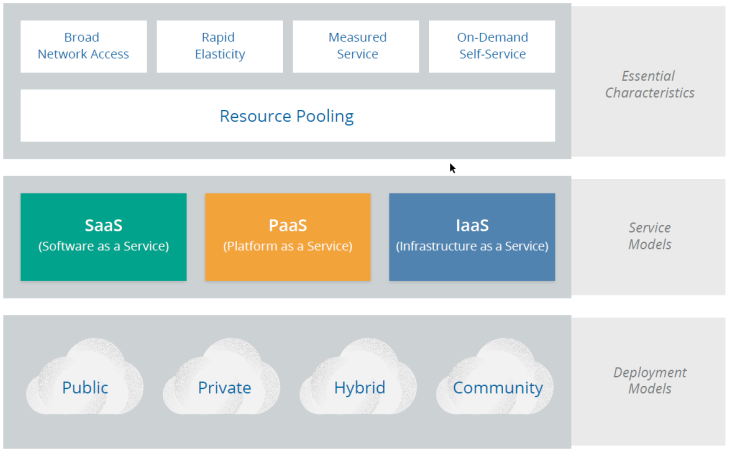
\includegraphics[width=\columnwidth]{cloud-services-1.png}

\subsection{Characteristics of a Cloud}
\begin{itemize}
\item Resource pooling is the most fundamental characteristic, as discussed above. The
provider abstracts resources and collects them into a pool, portions of which can be
allocated to different consumers (typically based on policies).
\item Consumers provision the resources from the pool using on-demand self-service.
They manage their resources themselves, without having to talk to a human
administrator.
\item Broad network access means that all resources are available over a network,
without any need for direct physical access; the network is not necessarily part of
the service.
\item Rapid elasticity allows consumers to expand or contract the resources they use
from the pool (provisioning and deprovisioning), often completely automatically. This
allows them to more closely match resource consumption with demand (for
example, adding virtual servers as demand increases, then shutting them down
when demand drops).
\item Measured service meters what is provided, to ensure that consumers only use what
they are allotted, and, if necessary, to charge them for it. This is where the term
utility computing comes from, since computing resources can now be consumed like
water and electricity, with the client only paying for what they use.
\end{itemize}

\subsection{Cloud Services}
\begin{itemize}
\item Software as a Service (SaaS) is a full application that’s managed and
hosted by the provider. Consumers access it with a web browser,
mobile app, or a lightweight client app.
\item Platform as a Service (PaaS) abstracts and provides development or
application platforms, such as databases, application platforms (e.g. a
place to run Python, PHP, or other code), file storage and
collaboration, or even proprietary application processing (such as
machine learning, big data processing, or direct Application
Programming Interfaces (API) access to features of a full SaaS
application). The key differentiator is that, with PaaS, you don’t
manage the underlying servers, networks, or other infrastructure.
\item Infrastructure as a Service (IaaS) offers access to a resource pool of
fundamental computing infrastructure, such as compute, network, or
storage.
\end{itemize}

\subsection{Cloud Services Security}
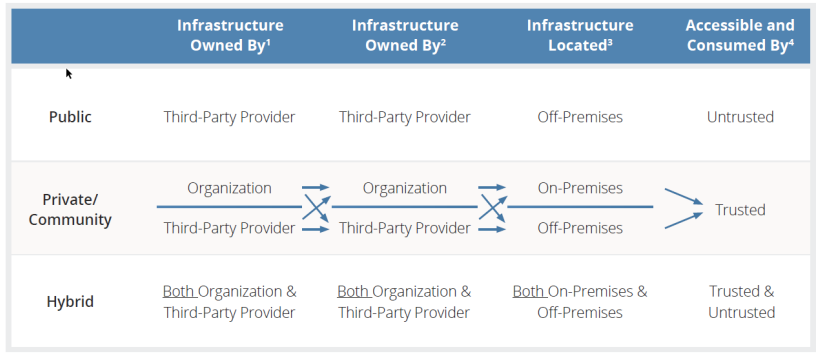
\includegraphics[width=\columnwidth]{cloud-service-security.png}

\subsection{Reference Architecture}
\begin{center}
    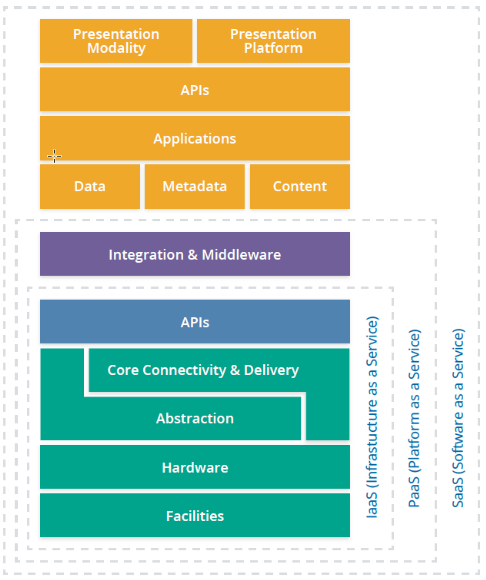
\includegraphics[width=0.6\columnwidth]{cloud-services-reference-arch.png}
\end{center}

\subsection{Simplified IaaS platform}
\begin{center}
    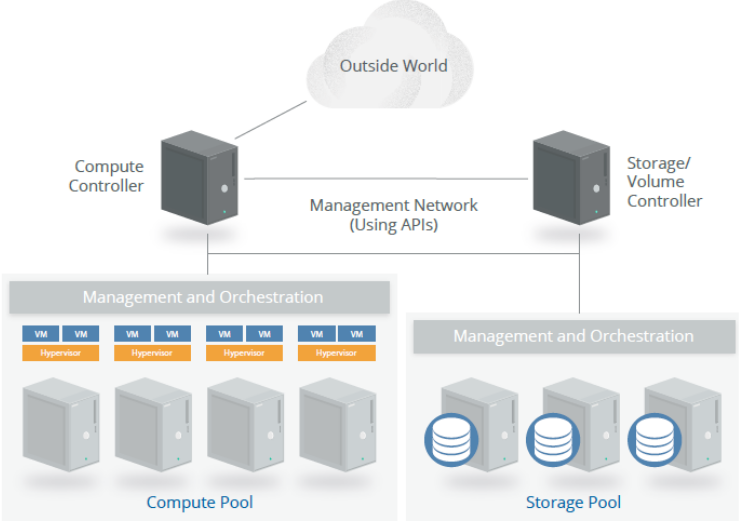
\includegraphics[width=\columnwidth]{cloud-simplified-iaas.png}
\end{center}

\subsection{Simplified SaaS on top of our IaaS}
\begin{center}
    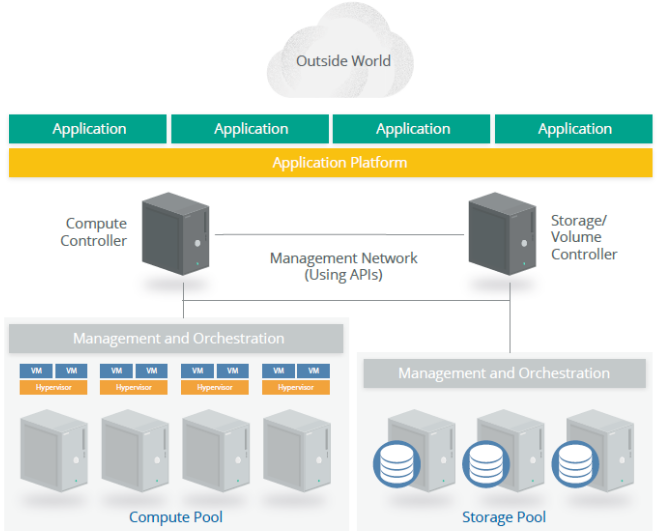
\includegraphics[width=\columnwidth]{cloud-simplified-saas.png}
\end{center}


\section{Capacity Planning}
As its name implies, the systems management discipline of capacity planning involves the planning of various kinds
of resource capacities for an infrastructure. \\
Capacity planning is a process to predict the types, quantities, and timing of critical resource capacities that are 
needed within an infrastructure to meet accurately forecasted workloads.\\
\subsection{4 Key Elements}
\begin{enumerate}
    \item The type of resource capacities required, such as servers, disk space, or bandwidth
    \item The size or quantities of the resource in question
    \item The exact timing of when the additional capacity is needed
    \item Decisions about capacity that are based on sound, thorough forecasts of anticipated workload demands
\end{enumerate}

\subsection{Why Capacity Planning Is Seldom Done Well}
\begin{enumerate}
    \item Analysts Are Too Busy with Day-To-Day Activities
    \item Users Are Not Interested (or able?) in Predicting Future Workloads
    \item Users Who Are Interested Cannot Forecast Accurately
    \item Capacity Planners May Be Reluctant to Use Effective Measuring
    Tools
    \item Need for updates: Corporate or IT Directions May Change over
    time (e.g. yearly)
    \item Planning Is Typically Not Part of an Infrastructure Culture
    \item Managers Sometimes Confuse Capacity Management with Capacity Planning
\end{enumerate}

\subsection{Steps to develop an effective capacity planning process}
\begin{enumerate}
    \item Select an Appropriate Capacity Planning Process Owner
    \item Identify the Key (Critical?) Resources to be Measured
    \item Monitor the Utilizations or Performance of the Resources
    \item Compare Utilizations to Maximum Capacities
    \item Collect Workload Forecasts from Developers and Users
    \item Transform Workload Forecasts into IT Resource Requirements
    \item Map Requirements onto Existing Utilizations
    \item Predict When the Business/Company Will Be Out of Capacity
    \item Update Forecasts and Utilizations
\end{enumerate}

\subsection{Additional Benefits of Capacity Planning}
\begin{enumerate}
    \item Strengthens Relationships with Developers and End-Users
    \item Improves Communications with Suppliers
    \item Encourages Collaboration with Other Infrastructure Groups
    \item Promotes a Culture of Strategic Planning as Opposed to Tactical Firefighting
\end{enumerate}

\subsection{Helpful Hints for Effective Capacity Planning}
\begin{enumerate}
    \item Start Small
    \item Speak the Language of Your Customers
    \item Consider Future Platforms
    \item Share Plans with Suppliers
    \item Anticipate Nonlinear Cost Ratios
    \item Plan for Occasional Workload Reductions
    \item Prepare for the Turnover of Personnel
    \item Strive to Continually Improve the Process
    \item Evaluate the Hidden Costs of Upgrades
\end{enumerate}

\subsection{Uncovering the Hidden Costs of Upgrades}
\begin{enumerate}
    \item Hardware Maintenance
    \item Technical Support
    \item Software Maintenance
    \item Memory Upgrades
    \item Channel Upgrades
    \item Cache Upgrades
    \item Data Backup Time
    \item Operations Support
    \item Offsite Storage
    \item Network Hardware
    \item Network Support
    \item Floor Space
    \item Power and Air Conditioning
\end{enumerate}

\subsection{Assessing an Infrastructure’s Capacity Planning Process}
\subsection{Measuring and Streamlining the Capacity Planning Process}
We can measure the effectiveness of a capacity planning process with service metrics such as the number of instances of 
poor response due to inadequate capacity on servers, disk devices, or the network. 
Process metrics—such as the number of instances of poor response due to inadequate capacity on servers, disk devices, 
or the network—help us gauge the efficiency of this process. 
We can be streamline the capacity planning process by automating certain actions—the notification to analysts when 
utilization thresholds are exceeded, the submittal of user forecasts, and the conversion of user-workload forecasts 
into capacity requirements, for example.

\section{Strategic Security}
Strategic security is designed to safeguard the availability, integrity, and confidentiality of designated data
 and programs against unauthorized access, modification, or destruction.

\subsection{Developing a Strategic Security Process}
\begin{enumerate}
    \item Identify an executive sponsor.
    \item Select a process owner.
    \item Define goals of strategic security.
    \item Establish review boards.
    \item Identify, categorize, and prioritize requirements.
    \item Inventory current state of security.
    \item Establish security organization.
    \item Develop security policies.
    \item Assemble planning teams.
    \item Review and approve plans.
    \item Evaluate technical feasibility of plans.
    \item Assign and schedule the implementation of plans.
\end{enumerate}

\subsection{Measuring and Streamlining the Security Process}
We can measure the effectiveness of a security process with service metrics such as the number of outages caused by 
security breaches and the amount of data altered, damaged, or deleted due to security violations. 
Process metrics, such as the number of password resets requested and granted and the number of multiple sign-ons 
processed over time, help us gauge the efficiency of this process. 
Finally, we can streamline the security process by automating certain actions—for example, the analysis of password 
resets, network violations, or virus protection invocations.

\section{Business Continuity}
Business continuity is a methodology to ensure the continuous operation of critical business systems in the event
of widespread or localized disasters to an infrastructure environment.

\subsection{Steps to Developing an Effective Business Continuity Process}
\begin{enumerate}
    \item Acquire executive support.
    \item Select a process owner.
    \item Assemble a cross-functional team.
    \item Conduct a business impact analysis.
    \item Identify and prioritize requirements.
    \item Assess possible business continuity recovery strategies.
    \item Develop a request for proposal (RFP) for outside services.
    \item Evaluate proposals and select the best offering.
    \item Choose participants and clarify their roles on the recovery team.
    \item Document the business continuity plan.
    \item Plan and execute regularly scheduled tests of the plan.
    \item Conduct a lessons-learned postmortem after each test.
    \item Continually maintain, update, and improve the plan.
\end{enumerate}

\section{Facilities Management}
Facilities management is a process to ensure that an appropriate physical environment is consistently supplied to 
enable the continuous operation of all critical infrastructure equipment.
\subsection{Major Elements}
\paragraph{UPS} uninterruptible power supply and is a temporary battery backup in the event of commercial power loss.
UPS units are normally used to power data centers for 15-20 minutes until such time that commercial power is restored 
or until longer term backup generators come online. 
Portable UPS units are now available for servers, workstations and desktops outside of a data center.

\subsection{Facilities Management Process Owner}
\begin{itemize}
    \item Determining the Scope of Responsibilities of a Facilities Management Process Owner
    \item Desired Traits of a Facilities Management Process Owner
\end{itemize}
The owner of the facilities management process almost always resides in the computer operations department.

\subsection{Evaluating the Physical Environment}
\begin{itemize}
    \item Major Physical Exposures Common to a Data Center
    \item Keeping Physical Layouts Efficient and Effective
\end{itemize}
If the problem-management system includes a robust database, it should be easy to analyze trouble tickets caused by 
facilities issues and highlight trends, repeat incidents, and root causes.

\subsection{Tips to Improve the Facilities Management Process}
\begin{enumerate}
    \item Nurture relationships with facilities department.
    \item Establish relationships with local government inspecting agencies, 
        especially if you are considering major physical upgrades to the data center.
    \item Consider using video cameras to enhance physical security.
    \item Analyze environmental monitoring
        reports to identify trends, patterns, and relationships.
    \item Design adequate cooling for hot spots due to concentrated equipment.
    \item Check on effectiveness of water and fire detection and suppression systems.
    \item Remove all tripping hazards in the computer center.
    \item Check on earthquake preparedness of data center
        (devices anchored down, training of personnel, and tie-in to disaster recovery).
\end{enumerate}
\subsection{Facilities Management at Outsourcing Centers}
Shops that outsource portions of their infrastructure services—co-location of servers is an example—often feel that the 
responsibility for the facilities management process is also outsourced and no longer of their concern. 
While outsourcers have direct responsibilities for providing stable physical environments, the client has an 
indirect responsibility to ensure this will occur. 
During the evaluation of bids and in contract negotiations, appropriate infrastructure personnel should ask the same 
types of questions about the outsourcer’s physical environment that they would ask if it were their own computer center.
\subsection{Measuring and Streamlining the Facilities Management Process}
We can measure the effectiveness of a facilities management process with service metrics such as the number 
of outages due to facilities management issues and the number of employee safety issues measured over time. 
Process metrics—for example, the frequency of preventative maintenance and inspections of air conditioning, 
smoke detection, and fire suppression systems and the testing of uninterruptible power supplies and backup 
generators—help us gauge the efficiency of this process. And we can streamline the facilities management process by 
automating actions such as notifying facilities personnel when environmental monitoring thresholds are exceeded 
for air conditioning, smoke detection, and fire suppression.

\section{IT Monitoring}
\begin{center}
    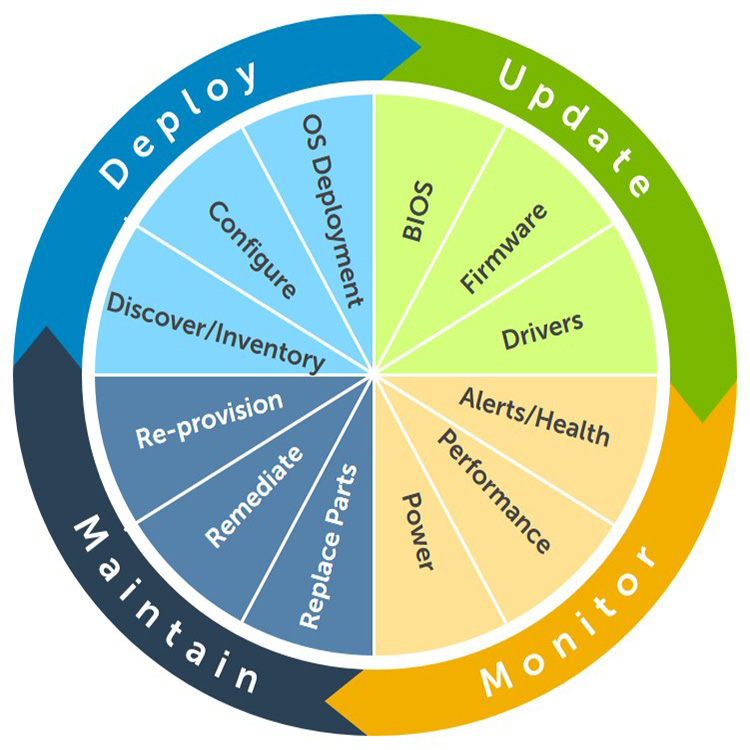
\includegraphics[width=4cm]{dell-lc-management.jpg}
\end{center}
\subsection{Ten Priorities for Systems Management}
\paragraph{Operating System Performance and Availability}
Monitoring processes should begin with the initial deployment
of an OS, ensuring the installation was a success or identifying any errors. The ongoing availability
of an OS must also be recorded and tracked by monitoring resources such as uptime and identifying
the failover status of clustered servers. OS performance must be monitored in real-time by recording
the status of system resources, including the load on CPUs, memory, and individual processes. Any
system performance elements that exceed established thresholds need to be immediately reported
to IT operations for prompt remediation. It is also essential to correlate OS performance with the
performance of applications and other workloads. In particular, database performance issues (identified
in error logs and job status reporting) can be difficult to resolve without mapping the issues to the
performance of system resources (such as CPU and memory status).

\paragraph{Server Hardware Status} All devices in a support stack must also be monitored to ensure their
physical hardware components are functioning optimally. Wear-and-
tear from continuous use and environmental conditions can degrade
a system’s performance or cause it to fail outright. Catching potential
hardware problems early will enable administrators to repair systems that
are failing or move workloads to new systems before the issues become
business impacting. Hardware components to monitor include the CPU,
memory SIMMs, USB ports, and SCSI chains. Administrators should
also be aware of which physical cable ports are in use and the status of
any additional direct-attached devices.

\begin{quote}
Catching potential hardware problems early will enable administrators to repair systems that are failing or 
move workloads to new systems before the issues become business impacting.
\end{quote}


\paragraph{Data and Storage Availability}
Another key pillar in systems management is ensuring the high performance and availability of
storage systems. This includes monitoring disk I/O performance, disk usage, and the integrity of the
file systems. Paging and swapping metrics are also important to track, especially for environments
that support dynamic data management systems, such as large SQL databases. Any storage devices
that include RAID technology must also be monitored and alarmed so any faulty drives can be
immediately replaced to ensure uninterrupted service. Storage Area Networks (SAN) and Network-
Attached Storage (NAS) also require vigilant monitoring to ensure data is being transmitted reliably
between storage devices.

\paragraph{Directory Services} 
Directory services (including Active Directory, LDAP, NIS, and DNS) provide centralized management
and distribution capabilities for critical system, network, and user information that are commonly
accessed by endpoints across the support stack. To ensure directory services are always accurate and
up to date, all changes (adds, deletes and updates) must be tracked and reported. This includes
monitoring for changes to both individual and group of users and systems. Details on change events
should be tracked to add accountability to directory service management processes. These include the
identification of who made the change and when it was made.

\paragraph{Patches and Updates}
All server software components – including operating systems, applications, drivers, and firmware –
require periodic patching and updates to new editions. These are often released to resolve performance
issues, security vulnerabilities, or code bugs, and are typically provisioned by IT operations. Since
it is essential to ensure that all software elements are promptly updated to ensure their security and
reliability, the availability of new patches and updates must be continuously tracked and then compared
against the versions currently installed on all devices in the support stack. By alarming on patches and
updates that need to be installed, administrators can quickly deploy the fixes, minimizing business
risks. Further, the patch deployment process itself must be monitored to assure they are successfully
installed. The date and time when patches were installed should also be recorded so they can later
be correlated with any system performance issues that may have resulted. This allows administrators
to rollback faulty patches before they become business impacting.

\paragraph{Virtualization Infrastructure Performance}
Virtualization continues to see increased adoption as a key enabler of cloud computing; however, the
complexity of the resources necessary for enabling a virtualized environment has also radically increased
management challenges. These difficulties can be broadly mitigated with the assistance of monitoring
and analytics, which should be employed in support of all types of virtualization – including server
virtualization, desktop virtualization, and application virtualization. Performance of each VM should
be recorded in a similar way to how it would be recorded on a static server, and alerts should be
activated if/when performance falls below established thresholds. However, VMs must also be mapped
to physical infrastructures and to any software dependencies necessary for their operations. In this way,
a failure or performance issue within a VM can be traced back to the physical component that is the
root cause of the problem.

\paragraph{Problem and Incident Alarming and Reporting}
Despite all preventative measures, sometimes failures and performance errors will occur in any IT
implementation. Incident management processes include the necessary procedures for detecting and
responding to issues that have already occurred. The key to effective incident management is prompt
identification of the failure – the faster it is identified, the faster it will
be resolved. The entire support stack (including hardware, software, and virtual components) must be continuously 
monitored so administrators can be immediately alerted to failure events. Some critical areas to monitor include: 
system logs, application and script status reports, threshold breach alerts, process tables 
(e.g. to identify hung or zombie processes) and database error logs.
To ensure administrators are not overwhelmed with requests, they should only be alerted to incidents that are business
impacting.

\begin{quotation}
    \noindent
The key to effective incident management is prompt identification of the failure – the faster it is identified, 
the faster it will be resolved.
\end{quotation}


\paragraph{Change Detection and Behavioral analysis}
Both proactive problem management and reactive incident resolution are improved with addition of
change detection. Nearly all IT failure events are caused by a change that was made to the environment
(the only exception to that rule being hardware failures caused by normal wear-and-tear), so by
identifying changes as they occur, failure events can be correlated to it and the root cause more rapidly
identified. All configuration elements should be monitored for change – including OS kernel and
system files, registry files, scripts, and applications – and records on each change event should include
what was changed, when it was changed, and who implemented the change. The latter adds an element
of accountability, allowing administrators to track back to who was responsible and determine why the
change was made. Of course, IT operations teams do not have the time to evaluate every change event,
so analytics should be in place to only alert them to changes that are impactful to the support stack.


\paragraph{Capacity Planning}
In order to ensure the continuous availability of IT services to support business requirements, IT
operations must proactively predict and promptly implement expansions to the capacity of IT resources.
For instance, when servers regularly exceed about 80\% of their capacity – in terms of CPU utilization,
memory performance, and storage availability – they should be upgraded or replaced. Storage capacity
should be identified by the amount of unallocated space, the amount of unused space in each partition,
and the overall I/O performance of the storage device or array. Similarly, organizations that support
virtualization implementations must monitor their capacity to support the existing number of VMs
and the expected number of new VMs that will be provisioned. Database capacities must also be
monitored by IT operations to ensure the system resources will be continuously available to support
them. This includes monitoring database and log file sizes, buffer mangers, caches, and the number of
active database user connections or open sessions.

\paragraph{Email Server Monitoring}
Email is an essential method of communication for any modern enterprise, which is why ensuring the
uninterrupted routing of email messages is also a top priority for IT operations. Email servers, such as
Microsoft Exchange, must be monitored to ensure they are continuously online and functioning at peak
performance. This includes monitoring to ensure all applicable protocols for outgoing mail (such as
SMTP) and incoming mail (such as POP3 and IMAP) are properly functioning, and the performance
of mail routing can be determined by tacking the round trip time of messages. Any mail routing failures
or performance issues should be logged and correlated to determine if the cause is a common system
error. Additionally, the messages themselves should be monitored to ensure they conform to enterprise
policies. Any emails with inappropriate content should be blacklisted and any messages sent from a
questionable source (identified by their IP address and domain names) should be blocked.

\subsection{Top 5 priorities for network security}
\paragraph{Identity and Access Management (IAM)}
Provide structure and reporting for authentication services
for personnel and systems throughout the enterprise.
\paragraph{Vulnerability Management} Identify and address vulnerabilities across all enterprise systems
and applications.
\paragraph{Change Monitoring} Identify changes, both authorized and unauthorized, to your infrastruc-
ture and who performed them.
\paragraph{Correlated, Centralized Event Management and Analysis} Maintain continuous monitoring
for anomalous, unusual, noncompliant, and malicious activities with a centralized repository for
collecting and displaying all recorded events with out-of-the-box and user customizable intel-
ligence and reporting.
\paragraph{Incident Response} Regularly updated and tested conglomeration of documented manual and
automated response processes and procedures available to the security personnel.


\subsection{Seven Priorities for Network Management}
\paragraph{Get the Network Under Management} In order to establish
effective network monitoring, the first step is to figure out which devices comprise the network and what
critical resources are connected to it and by it. You can’t manage what you don’t know is out there, and
EMA has heard countless stories of surprises resulting from initial (or even ongoing) network discovery.
Start by selecting a network monitoring product. Some are simple, and some are sophisticated, but they
all allow the collection of network device information for bringing devices under management.
\\
There are a number of critical connected resources that
should also be incorporated as part of the initial monitoring push:
\begin{itemize}
    \item Network-enabling resources, such as DNS (Domain Name Service) and AD (Active Directory)
    servers, as well as IP address management systems such as DHCP (Dynamic Host Control
    Protocol), should be defined or discovered and added. These services are critical to basic network
    functionality, and when any of them stop functioning properly, network and application health
    and performance suffers. For instance, if AD authentication is not occurring because the server is
    down, users will not be able to access their Exchange email.
    \item Network security elements such as firewalls and IDS/IPSs (Intrusion Detection/Prevention
    Systems) will commonly sit in-line as part of the network path.
    \item Critical connected application servers are important too. You want to know that those systems are
    up, and at the very least that their Network Interface Cards (NICs) are functioning properly, so
    they can access the network without problems.
\end{itemize}
\paragraph{Define Device Groupings}
The next step is to organize the elements to be monitored. This essential step allows network monitoring teams to 
designate the relative importance of each component, according to specific characteristics of the organization and
the managed infrastructure. Basically, the goal of this step is to link the monitored network to the
organization that it connects and supports. \\
\\
There are three types of grouping approaches that EMA finds to be most common and useful across
settings both large and small, and using them helps to answer the what, where, and who of problem
isolation and management. Following are some key types:
\begin{itemize}
    \item Device Type: Network managers most often start with views into the managed network that bring
    together devices by category, such as routers, switches, and access points. This approach to grouping
    facilitates inventory management, device administration, and general health assessments. This will
    often be the place to figure out precisely what is the source of a problem under investigation.
    \item Geographical: For any organization that has more than one operating location, a geographical or
    site-based grouping of monitored devices is perhaps the most easily understandable way of looking
    at the network. This answers the question of where problems have occurred. Graphical topology
    map views fill this need and are often used as a primary display in the NOC (Network Operations
    Center) as a visual guide to operations status. It is also very helpful for quickly isolating the scope
    and impact of any problem.
    \item Organizational: The most direct technique for relating network monitoring information to the
    connected community is to group network elements in terms of which part of the business or
    organization they serve. This addresses the question of who is impacted by any issue or problem.
    There will be a lot of overlap here, when considering core devices, but this is key to recognizing and
    accurately communicating with end-user and line of business communities, whether for regular
    status reporting or during a troubleshooting and recovery scenario.
\end{itemize}

\paragraph{Prioritized Availability Monitoring}
The next step and priority is to define which devices, groups, and/or sites are to be designated as most
critical to the organization. Any time one of these switches or ports is down unexpectedly, it’s likely
that access to important applications has been interrupted or, at best, impaired. These will be the
network components that will be assigned the highest priority for sustained monitoring – when any of
these elements or locations suffers an availability incident, they will receive priority attention from the
operations staff.

\paragraph{Add Device-level Performance Monitoring}
With availability monitoring in hand, network managers can turn towards the next major set of
challenges – recognizing and managing the performance of the network. The objective here is to move
beyond being able to answer the question “is the network up?” and onto “is the network meeting
performance and throughput expectations?” The most common mechanism for this is to expand
availability-oriented SNMP polling to collect a broad range of health and activity metrics from network
devices on a repeating periodic basis. That data is then archived and kept in a historical database, so that
trends can be identified and normal versus abnormal activity revealed.
Following are a set of essential areas to focus upon for establishing device-level network performance monitoring:
\begin{itemize}
    \item Monitoring device resources: Collecting metrics on current levels of device resources such as
    CPU usage, memory usage, power levels, temperature (and more) reveals a detailed view of the
    operational capacity and health of each device.
    \item Monitoring ports/interfaces: By harvesting counters such as packets, octets, discards and errors
    both coming into and going out of each logical and physical interface, it is possible to recognize
    congestion issues as well as operational viability of the many touch points that comprise the
    connectivity fabric.
    \item Setting performance thresholds: Default performance alerts/alarms should be configured to watch
    for extreme high values in monitored metrics across all devices, such as interface utilization or
    device CPU exceeding 90\%, and tuned more finely for critical/essential devices and resources.
    This provides indications to network managers that network links may be approaching saturation,
    before the network begins to fail.
    \item Identifying trends: Your monitoring system should provide reports on performance metrics over
    time so that you can recognize trends over weeks, months, or even the past year. This provides
    network engineering the data necessary to accurately plan capacity, and network managers the
    ability to recognize changes in usage patterns or quality indicators that warrant proactive mitigation.
\end{itemize}

\paragraph{Get Change Under Control}
Enemy number one, when it comes to stability and performance of the
network, is unplanned change or unintended consequences of change.
Consequently, an essential aspect of monitoring networks for both
performance and health must include recognition of changes being made
to the network or occurring within the network. For instance, a routing
change can break a network path between sites, a network QoS tag could
be misconfigured and starve a latency-sensitive application like VoIP of
necessary priority delivery, or a firewall rule change could block access to
a critical application. Having change indicators on hand can significantly
accelerate both problem troubleshooting as well as remediation. \\
\\
There are two techniques for integrating change awareness into network monitoring. The first involves
finding and capturing change indicators, and adding them into the primary monitoring platform and
process. These indicators can often be found in the form of device traps or notifications (sometimes via
API). Another good source is log files, where the exact change made, the time it was made, and often
who made the change is captured and recorded. \\
The second important approach for establishing control over change is to leverage the ability of NCCM
(Network Change and Configuration Management) tools to automatically scan devices, compare their
configurations to expected norms, and automatically report variances. This latter approach can help
reveal potential problem sources while also providing the added value of assuring policy and regulatory
compliance. NCCM tools may be available as a module that works directly with your network monitoring
platform, which will be easiest to integrate into monitoring practices, or may be stand-alone in nature, in
which case a bit more effort will be needed to incorporate change indicators and scan results.
\paragraph{Add Application Awareness}
With the network layer well in hand, being monitored for availability, performance, and change,
network managers can turn their focus upon adding the crown jewel of monitoring – application
awareness. The objective here is to understand exactly what is traveling over the network, from where to
where, in what volumes, and at what times. This is the touch point between a network and the served
organization, yielding direct insight into the applications and services that the network is entrusted and
expected to deliver. It also represents one of the most direct opportunities
for recognizing how individuals as well as groups utilize and gain value
from the network. \\
With application-aware data incorporated into the monitoring process, measures can be taken to
leverage it in a manner similar to device-based performance outlined above. Network managers will
want to set thresholds so that they may be notified of unexpected spikes or high levels of activity of any
individual application or any individual end-user. Unexpectedly low levels of activity may also be of
interest, as it may be an indication of impaired application or transaction activity.
\paragraph{Integrate and Communicate}
The full value of network monitoring cannot be fully realized without sharing and collaborating,
both across the IT infrastructure team as well as beyond. Since the network is the fabric connecting
IT-empowered organizations, it represents a strategic viewpoint for understanding the ebb and flow of
activity and health of the IT function in the eyes of those who rely upon IT for their daily tasks and work.
That viewpoint is a powerful one that when effectively shared, and can facilitate improved planning,
smoother rollouts, and a better collective understanding of operations between IT and their customers. \\
Following are recommended focus areas for integration and sharing of information into and from the network 
monitoring function:

\begin{itemize}
    \item \textbf{Help desk and trouble ticketing}: Connecting the network monitoring system to a trouble ticketing
    platform, and/or directly into a help desk management system, provides a link for tracking issues
    as they arise, the steps that have been taken to remedy them, in the final dispensation. Time-based
    escalation procedures can also be automated for network issues using the features in these systems,
    providing a better experience for IT’s customers.
    \item \textbf{Systems and application monitoring}: The network connects systems to end users or to other systems,
    to deliver application and service traffic. By aligning network monitoring with monitoring of systems
    and applications, IT operations teams can correlate indicators and events to recognize dependencies
    and accelerate identification of root causes. This may involve another layer of management technology,
    to serve as a central consolidation point, or may be possible within the core network management
    platform, if that system has been designed to incorporate data from other domains.
    \item \textbf{Security monitoring and management}: Many of the technologies and data sources used for
    network security monitoring are the same as those used for network operations monitoring. Issues
    recognized within the network may, at times, actually reflect security threats. Open sharing of
    activity and issues found by the network monitoring team with the security team can greatly
    accelerate incident assessment and remediation. As with systems and applications, this may involve
    forwarding of events or data to a central SEIM (Security Event and Information Management)
    platform, or may be an integral capability of the network monitoring system.
    \item \textbf{Line of business and end users}: Finally, we cannot forget those who the network serves. Providing
    a means for reporting or exposing current network health, availability, and even performance
    status to senior executive leadership and even down to end users can be very helpful in managing
    expectations and proving value delivered. Essential here is the ability to focus reporting upon that
    portion of the infrastructure that is relevant to a user, group of users, or line of business, so that
    they are not overloaded with information that is not pertinent to their needs.
\end{itemize}

\subsection{80\% Rule}
When servers regularly exceed about 80\% of their capacity – in terms of CPU utilization, memory performance, 
and storage availability – they should be upgraded or replaced. 

\section{CoBIT Framework}
COBIT (Control Objectives for Information and Related Technologies) is a good-practice framework created by 
international professional association ISACA for information technology (IT) 
management and IT governance. COBIT provides an implementable "set of controls over information technology and organizes
them around a logical framework of IT-related processes and enablers."

The business orientation of COBIT consists of linking business goals to IT goals, providing metrics and maturity models
to measure their achievement, and identifying the associated responsibilities of business and IT process owners.
The process focus of COBIT is illustrated by a process model that subdivides IT into four domains 
(Plan and Organize; Acquire and Implement; Deliver and Support; and Monitor and Evaluate) and 34 processes inline with 
the responsibility areas of plan, build, run, and monitor. It is positioned at a high level and has been aligned and 
harmonized with other, more detailed IT standards and good practices such as COSO, ITIL, BiSL, ISO 27000, CMMI, TOGAF 
and PMBOK. COBIT acts as an integrator of these different guidance materials, summarizing key objectives under one 
umbrella framework that link the good practice models with governance and business requirements.
COBIT 5 further consolidated and integrated the COBIT 4.1, Val IT 2.0 and Risk IT frameworks and drew from ISACA's IT 
Assurance Framework (ITAF) and the Business Model for Information Security (BMIS).

The framework and its components can, when utilized well, also contribute to ensuring regulatory compliance.
It can encourage less wasteful information management, improve retention schedules, increase business agility, and 
lower costs while better complying with data retention and management regulations. \\
\\
COBIT components include:\\
\begin{itemize}
    \item \textbf{Framework}: Organizes IT governance objectives and good practices by IT domains and processes and links them to business requirements.
    \item \textbf{Process descriptions}: A reference process model and common language for everyone in an organization. The processes map to responsibility areas of plan, build, run, and monitor.
    \item \textbf{Control objectives}: Provides a complete set of high-level requirements to be considered by management for effective control of each IT process.
    \item \textbf{Management guidelines}: Helps assign responsibility, agree on objectives, measure performance, and illustrate interrelationship with other processes.
    \item \textbf{Maturity models}: Assesses maturity and capability per process and helps to address gaps.
\end{itemize}



\begin{center}
    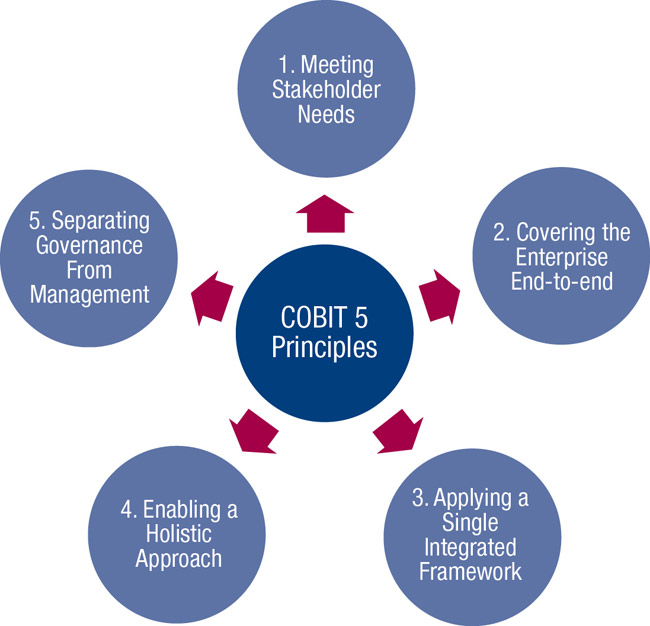
\includegraphics[width=4cm]{cobit-fw.jpg}\\
\end{center}
\noindent
The COBIT 5 framework defines
7 categories of enablers:
\begin{itemize}
    \item Principles, Policies and Frameworks
    \item Processes
    \item Organisational Structures
    \item Culture, Ethics and Behaviour
    \item Information
    \item Services, Infrastructure and Applications
    \item People, Skills and Competencies
\end{itemize}
\vspace{1em}
\noindent
The COBIT 5 framework makes a clear distinction between
governance and management. These two disciplines encompass
different types of activities, require different organisational structures
and serve different purposes. COBIT 5’s view on this key distinction
between governance and management is:

\begin{itemize}
    \item Governance ensures that stakeholder needs, conditions and options
    are evaluated to determine balanced, agreed-on enterprise objectives
    to be achieved; setting direction through prioritisation and decision
    making; and monitoring performance and compliance against
    agreed-on direction and objectives (e.g. board of directors).
    \item Management plans, builds, runs and monitors activities in alignment
    with the direction set by the governance body to achieve the
    enterprise objectives (e.g. CEO).
\end{itemize}

\subsection{Governance Objective: the value creation}
\begin{center}
    \begin{minipage}{0.5\columnwidth}
        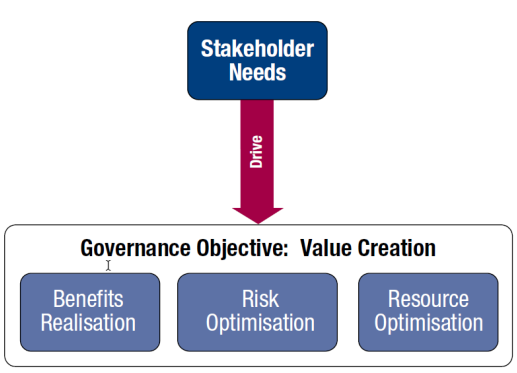
\includegraphics[width=\columnwidth]{governance-objective-value-creation.png}
    \end{minipage}
\end{center}

\subsection{Governance and Management in COBIT5}
\begin{center}
    \begin{minipage}{0.5\columnwidth}
        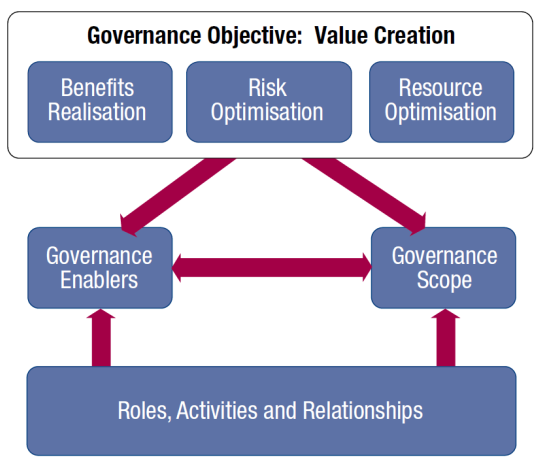
\includegraphics[width=\columnwidth]{governance-management-cobit5.png}
    \end{minipage}
\end{center}

\subsection{Key Roles, Activities and Relationships}
\begin{center}
    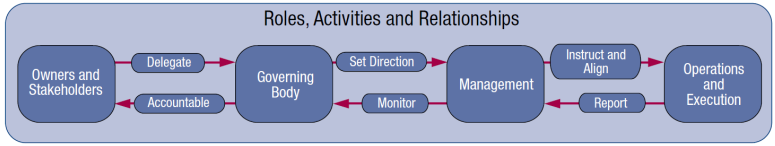
\includegraphics[width=\columnwidth]{cobit-key-roles.png}
\end{center}

\subsection{Enterprise Enablers}
\begin{center}
    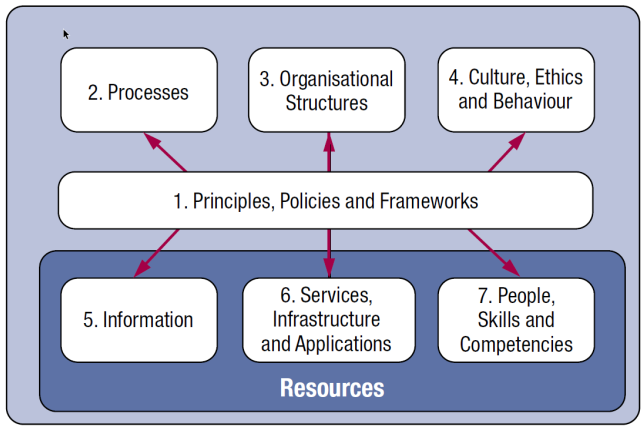
\includegraphics[width=\columnwidth]{cobit-enterprise-enablers.png}
\end{center}

\subsection{Enterprise Enablers (2)}
\begin{center}
    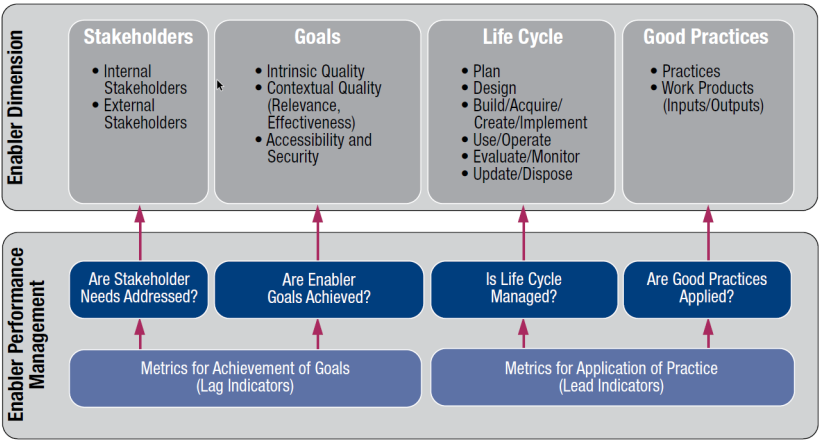
\includegraphics[width=\columnwidth]{cobit-enterprise-enablers-2.png}
\end{center}

\subsection{Management and Governance key areas and responsibilities}
\begin{center}
    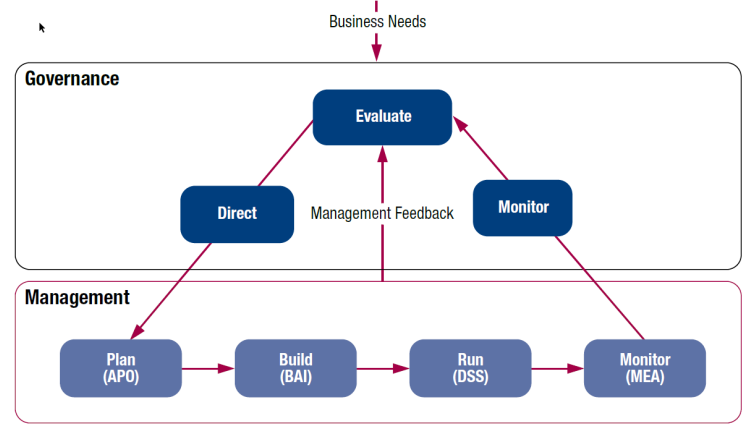
\includegraphics[width=\columnwidth]{cobit-management-governance-key-areas.png}
\end{center}

\subsection{Table of Maturity Levels}
\begin{center}
    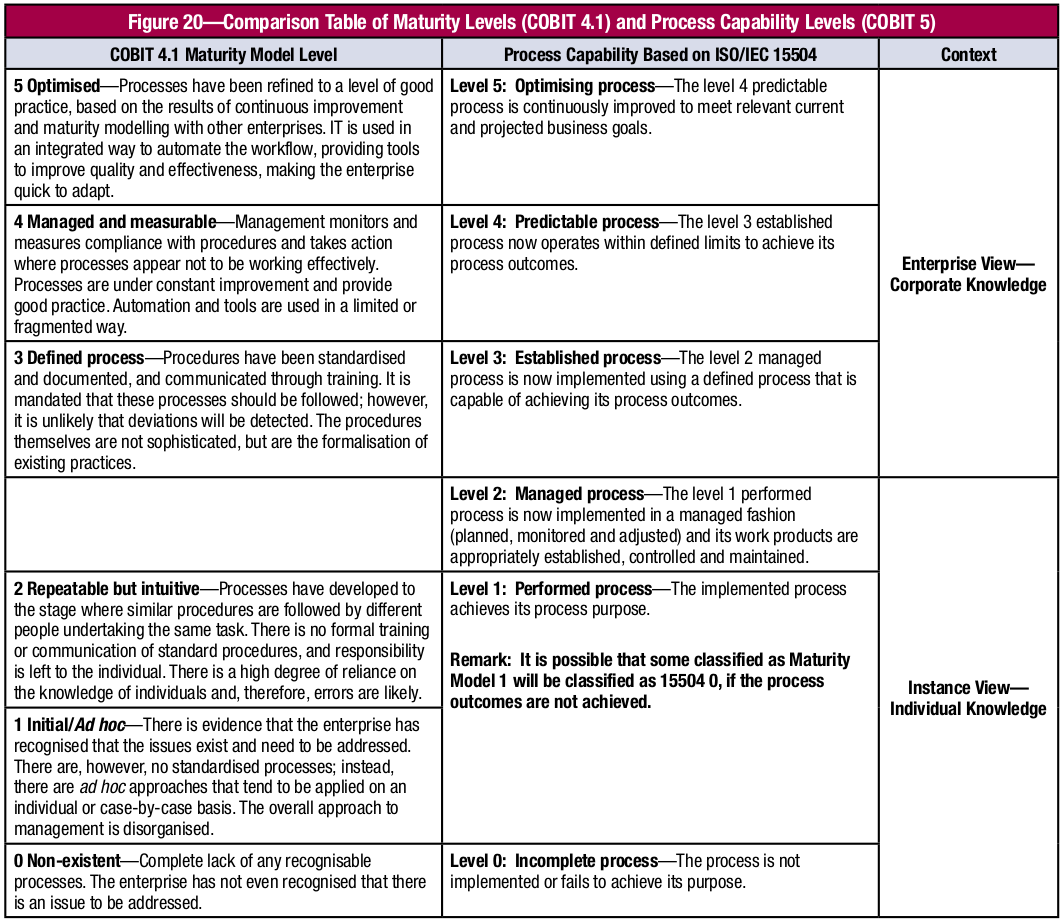
\includegraphics[width=\columnwidth]{cobit-maturity-level-comparison.png}
\end{center}


\subsection{Cobit 5 vs Cobit 4.1}
\begin{center}
    \begin{minipage}{\columnwidth}
        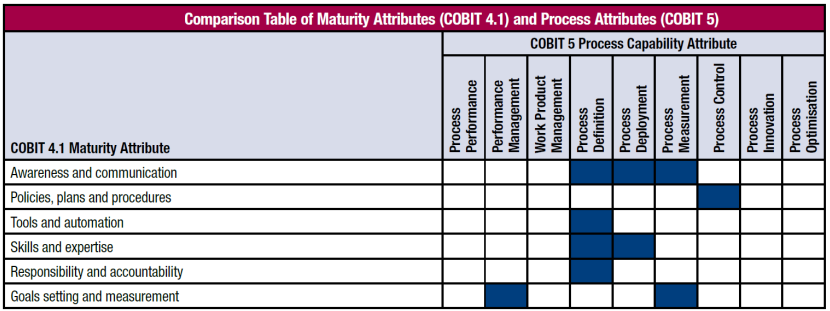
\includegraphics[width=\columnwidth]{cobit5-vs-cobit41.png}
    \end{minipage}
\end{center}

\subsection{ISACA}
Leading global provider of knowledge, certifications, community, advocacy, education on information systems (IS), 
assurance and security, enterprise governance and management of IT, IT-related risk and compliance.\\
95,000 constituents in 160 countries. ISACA attests IT skills \& knowledge through recognized certifications:
\begin{itemize}
    \item Certified Information Systems Auditor® (CISA®),
    \item Certified Information Security Manager® (CISM®),
    \item Certified in the Governance of Enterprise IT® (CGEIT®) and
    \item Certified in Risk and Information Systems ControlTM (CRISCTM) designations
\end{itemize}

\subsection{CoBIT 5: SIEM}
Security information and event management (SIEM), it is a solution enterprise security professionals both insight into
and a track record of the activities within their IT environment. It provides Real time analysis of log and event data,
to provide: 
\begin{itemize}
    \item threat monitoring,
    \item event correlation and
    \item incident response
\end{itemize}
\noindent
Collects and aggregates log data generated throughout the
organization’s technology infrastructure:
\begin{itemize}
    \item servers
    \item host systems
    \item applications
    \item network and
    \item security devices such as firewalls and antivirus filters.
\end{itemize}
\noindent
SIEM software identifies and categorizes incidents and events, as well as analyzes them. \\
SIEM has 2 main objectives:
\begin{itemize}
    \item providing reports on security-related incidents and events,
    such as successful and failed logins, malware activity and
    other possible malicious activities
    \item sending alerts if the event analysis discovers an activity that
    runs against predetermined rulesets, indicating a potential
    security issue.
\end{itemize}
\noindent
SIEM is implemented via software, systems, appliances, or some combination of these items. 
There are, generally speaking, six main attributes of an SIEM system:

\begin{itemize}
    \item \textbf{Retention}: Storing data for long periods so that decisions can be made off of more
    complete data sets.
    \item \textbf{Dashboards}: Used to analyze (and visualize) data in an attempt to recognize patterns
    or target activity or data that does not fit into a normal pattern.
    \item \textbf{Correlation}: Sorts data into packets that are meaningful, similar and share common
    traits. The goal is to \underline{turn data into useful information}.
    \item \textbf{Alerting}: When data is gathered or identified that trigger certain responses - such as
    alerts or potential security problems - SIEM tools can activate certain protocols to alert
    users, like notifications sent to the dashboard, an automated email or text message.
    \item \textbf{Data Aggregation}: Data can be gathered from any number of sites once SIEM is
    introduced, including servers, networks, databases, software and email systems. The
    aggregator also serves as a consolidating resource before data is sent to be
    correlated or retained.
    \item \textbf{Compliance}: Protocols in a SIEM can be established that automatically collect data
    necessary for compliance with company, organizational or government policies.
\end{itemize}

\subsection{6 Ways to screw up a SIEM implementation}
\begin{center}
    \begin{minipage}{\columnwidth}
        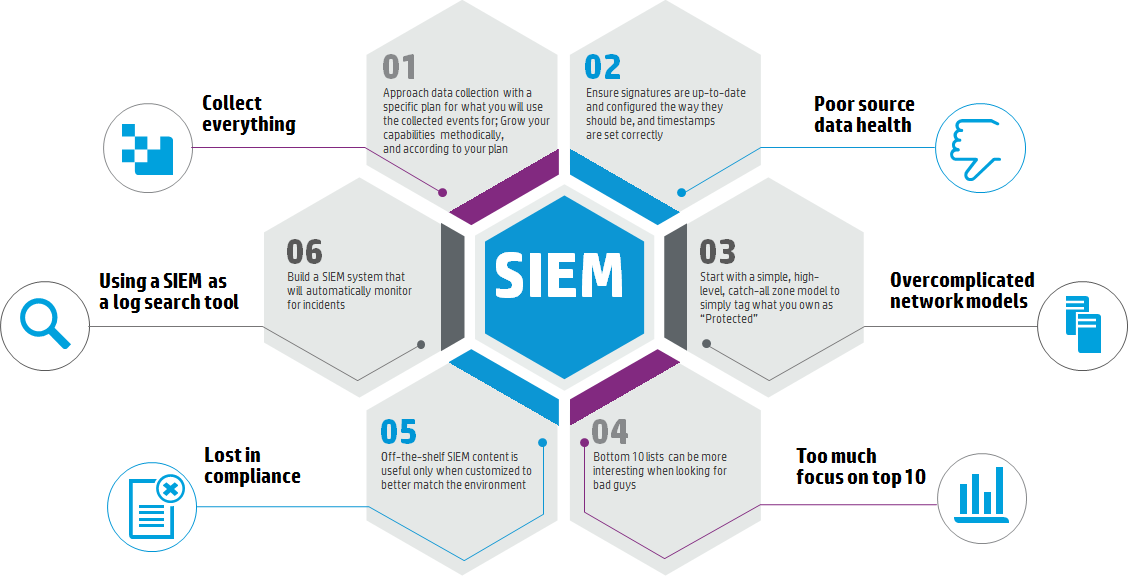
\includegraphics[width=\columnwidth]{screw-up-SIEM.png}
    \end{minipage}
\end{center}

\section{SOC}
An information security operations center ("ISOC" or "SOC") is a facility where enterprise information systems 
(web sites, applications, databases, data centers and servers, networks, desktops and other endpoints) 
are monitored, assessed, and defended. 

\subsection{High Level View}
\begin{center}
    \begin{minipage}{\columnwidth}
        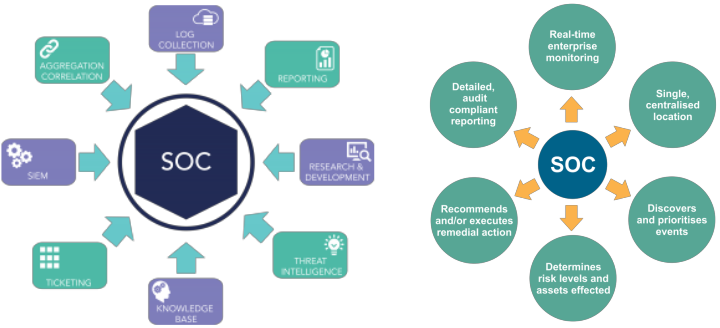
\includegraphics[width=\columnwidth]{soc-high-level.png}
    \end{minipage}
\end{center}

\subsection{Typical Services handled by SOC}

\begin{itemize}
    \item Security Monitoring \& Incident Handling
    \begin{itemize}
        \item Security Incident Handling
        \item New Threats Management
    \end{itemize}
    \item Operational Security Management
    \begin{itemize}
        \item Risk Analysisy Management (Security Plans)
        \item Remediation Plans
        \item Operational Security
    \end{itemize}
    \item Technical Security Analysis
    \begin{itemize}
        \item Vulnerability Assessment
        \item Security Baseline Compliance Assessment
        \item Forensics Analysis Services
    \end{itemize}
    \item Security Infrastructures Management
    \begin{itemize}
        \item Operational Security
    \end{itemize}
\end{itemize}
\noindent
SOC’s modular design enables adding/removing different services depending on organization requirements and
InfoSec maturity.

\subsection{SOC's Team Skills - General}
Synthetically, the SOC team manages and prevents security issues and defines all security instructions/guidelines
for IT teams and therefore requires a diverse and very high level of expertise grouped into 4 distinct areas 
of expertise.
\noindent
The SOC general skill-set are:
\begin{itemize}
    \item Security Skills
    \item Network Skills
    \item Infrastructure Skills
    \item Governance \& Compliance Skills
\end{itemize}

\subsection{SOC Options}
\begin{center}
    \begin{minipage}{\columnwidth}
        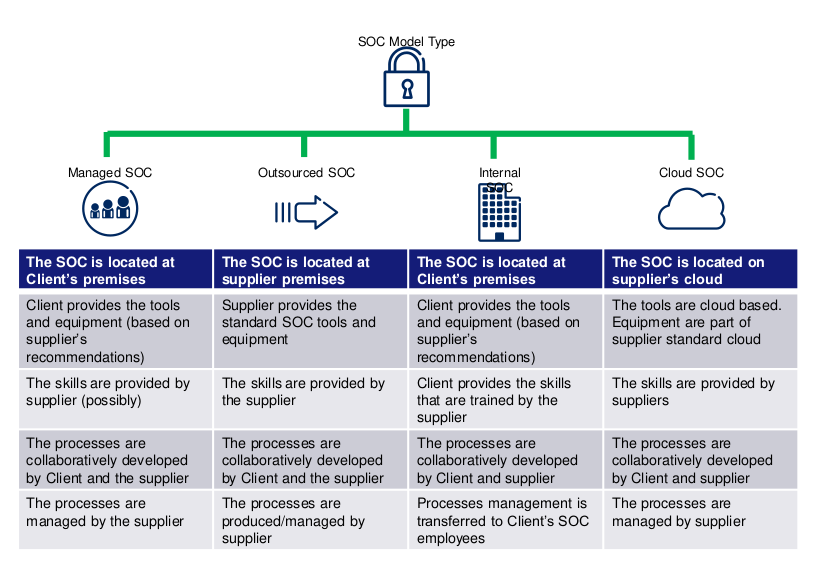
\includegraphics[width=\columnwidth]{soc-options.png}
    \end{minipage}
\end{center}


\section{SysAdmin Code Of Ethics}
We as professional System Administrators do hereby commit ourselves to the highest standards of
ethical and professional conduct, and agree to be guided by this code of ethics, and encourage every
System Administrator to do the same.

\paragraph{Professionalism} I will maintain professional conduct in the workplace and will not allow personal
feelings or beliefs to cause me to treat people unfairly or unprofessionally.
\paragraph{Personal Integrity} I will be honest in my professional dealings and forthcoming about my competence
and the impact of my mistakes. I will seek assistance from others when required.
I will avoid conflicts of interest and biases whenever possible. When my advice is sought, if I have a
conflict of interest or bias, I will declare it if appropriate, and recuse myself if necessary.
\paragraph{Privacy} I will access private information on computer systems only when it is necessary in the course of
my technical duties. I will maintain and protect the confidentiality of any information to which I may
have access, regardless of the method by which I came into knowledge of it.
\paragraph{Laws and Policies} I will educate myself and others on relevant laws, regulations,
and policies regarding the performance of my duties.

\paragraph{Communication} I will communicate with management, users, and colleagues about computer matters
of mutual interest. I will strive to listen to and understand the needs of all parties.
\paragraph{System Integrity} I will strive to ensure the necessary integrity, reliability, and availability of the systems
for which I am responsible.
I will design and maintain each system in a manner to support the purpose of the system to the
organization.
\paragraph{Education} I will continue to update and enhance my technical knowledge and other work-related skills.
I will share my knowledge and experience with others.
\paragraph{Responsibility to Computing Community} I will cooperate with the larger computing community to
maintain the integrity of network and computing resources.
Social Responsibility As an informed professional, I will encourage the writing and adoption of relevant
policies and laws consistent with these ethical principles.
\paragraph{Ethical Responsibility} I will strive to build and maintain a safe, healthy, and productive workplace.
I will do my best to make decisions consistent with the safety, privacy, and well-being of my community
and the public, and to disclose promptly factors that might pose unexamined risks or dangers.
I will accept and offer honest criticism of technical work as appropriate and will credit properly the
contributions of others.
I will lead by example, maintaining a high ethical standard and degree of professionalism in the
performance of all my duties. I will support colleagues and co-workers in following this code of ethics.
\end{multicols}
\end{document}